% Created by tikzDevice version 0.12.4 on 2023-11-10 09:29:53
% !TEX encoding = UTF-8 Unicode
\documentclass[10pt]{article}
\usepackage{tikz}
\usepackage{libertine}
\usepackage{amsmath}\begin{document}

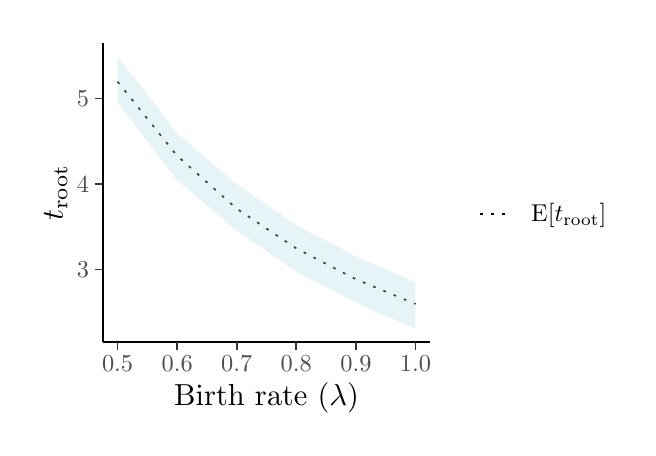
\begin{tikzpicture}[x=1pt,y=1pt]
\definecolor{fillColor}{RGB}{255,255,255}
\path[use as bounding box,fill=fillColor,fill opacity=0.00] (0,0) rectangle (216.81,144.54);
\begin{scope}
\path[clip] (  0.00,  0.00) rectangle (216.81,144.54);
\definecolor{drawColor}{RGB}{255,255,255}
\definecolor{fillColor}{RGB}{255,255,255}

\path[draw=drawColor,line width= 0.6pt,line join=round,line cap=round,fill=fillColor] (  0.00, -0.00) rectangle (216.81,144.54);
\end{scope}
\begin{scope}
\path[clip] ( 27.10, 30.86) rectangle (145.51,139.04);
\definecolor{fillColor}{RGB}{255,255,255}

\path[fill=fillColor] ( 27.10, 30.86) rectangle (145.51,139.04);
\definecolor{drawColor}{RGB}{0,0,0}

\path[draw=drawColor,line width= 0.6pt,dash pattern=on 1pt off 3pt ,line join=round] ( 32.49,125.01) --
	( 54.01, 98.24) --
	( 75.54, 79.12) --
	( 97.07, 64.77) --
	(118.60, 53.62) --
	(140.12, 44.70);
\definecolor{fillColor}{RGB}{173,216,230}

\path[fill=fillColor,fill opacity=0.30] ( 32.49,134.12) --
	( 54.01,106.25) --
	( 75.54, 87.96) --
	( 97.07, 73.18) --
	(118.60, 61.90) --
	(140.12, 52.56) --
	(140.12, 35.78) --
	(118.60, 45.12) --
	( 97.07, 56.41) --
	( 75.54, 71.18) --
	( 54.01, 89.47) --
	( 32.49,117.35) --
	cycle;

\path[] ( 32.49,134.12) --
	( 54.01,106.25) --
	( 75.54, 87.96) --
	( 97.07, 73.18) --
	(118.60, 61.90) --
	(140.12, 52.56);

\path[] (140.12, 35.78) --
	(118.60, 45.12) --
	( 97.07, 56.41) --
	( 75.54, 71.18) --
	( 54.01, 89.47) --
	( 32.49,117.35);
\end{scope}
\begin{scope}
\path[clip] (  0.00,  0.00) rectangle (216.81,144.54);
\definecolor{drawColor}{RGB}{0,0,0}

\path[draw=drawColor,line width= 0.6pt,line join=round] ( 27.10, 30.86) --
	( 27.10,139.04);
\end{scope}
\begin{scope}
\path[clip] (  0.00,  0.00) rectangle (216.81,144.54);
\definecolor{drawColor}{gray}{0.30}

\node[text=drawColor,anchor=base east,inner sep=0pt, outer sep=0pt, scale=  0.88] at ( 22.15, 54.25) {3};

\node[text=drawColor,anchor=base east,inner sep=0pt, outer sep=0pt, scale=  0.88] at ( 22.15, 85.16) {4};

\node[text=drawColor,anchor=base east,inner sep=0pt, outer sep=0pt, scale=  0.88] at ( 22.15,116.08) {5};
\end{scope}
\begin{scope}
\path[clip] (  0.00,  0.00) rectangle (216.81,144.54);
\definecolor{drawColor}{gray}{0.20}

\path[draw=drawColor,line width= 0.6pt,line join=round] ( 24.35, 57.13) --
	( 27.10, 57.13);

\path[draw=drawColor,line width= 0.6pt,line join=round] ( 24.35, 88.05) --
	( 27.10, 88.05);

\path[draw=drawColor,line width= 0.6pt,line join=round] ( 24.35,118.97) --
	( 27.10,118.97);
\end{scope}
\begin{scope}
\path[clip] (  0.00,  0.00) rectangle (216.81,144.54);
\definecolor{drawColor}{RGB}{0,0,0}

\path[draw=drawColor,line width= 0.6pt,line join=round] ( 27.10, 30.86) --
	(145.51, 30.86);
\end{scope}
\begin{scope}
\path[clip] (  0.00,  0.00) rectangle (216.81,144.54);
\definecolor{drawColor}{gray}{0.20}

\path[draw=drawColor,line width= 0.6pt,line join=round] ( 32.49, 28.11) --
	( 32.49, 30.86);

\path[draw=drawColor,line width= 0.6pt,line join=round] ( 54.01, 28.11) --
	( 54.01, 30.86);

\path[draw=drawColor,line width= 0.6pt,line join=round] ( 75.54, 28.11) --
	( 75.54, 30.86);

\path[draw=drawColor,line width= 0.6pt,line join=round] ( 97.07, 28.11) --
	( 97.07, 30.86);

\path[draw=drawColor,line width= 0.6pt,line join=round] (118.60, 28.11) --
	(118.60, 30.86);

\path[draw=drawColor,line width= 0.6pt,line join=round] (140.12, 28.11) --
	(140.12, 30.86);
\end{scope}
\begin{scope}
\path[clip] (  0.00,  0.00) rectangle (216.81,144.54);
\definecolor{drawColor}{gray}{0.30}

\node[text=drawColor,anchor=base,inner sep=0pt, outer sep=0pt, scale=  0.88] at ( 32.49, 20.14) {0.5};

\node[text=drawColor,anchor=base,inner sep=0pt, outer sep=0pt, scale=  0.88] at ( 54.01, 20.14) {0.6};

\node[text=drawColor,anchor=base,inner sep=0pt, outer sep=0pt, scale=  0.88] at ( 75.54, 20.14) {0.7};

\node[text=drawColor,anchor=base,inner sep=0pt, outer sep=0pt, scale=  0.88] at ( 97.07, 20.14) {0.8};

\node[text=drawColor,anchor=base,inner sep=0pt, outer sep=0pt, scale=  0.88] at (118.60, 20.14) {0.9};

\node[text=drawColor,anchor=base,inner sep=0pt, outer sep=0pt, scale=  0.88] at (140.12, 20.14) {1.0};
\end{scope}
\begin{scope}
\path[clip] (  0.00,  0.00) rectangle (216.81,144.54);
\definecolor{drawColor}{RGB}{0,0,0}

\node[text=drawColor,anchor=base,inner sep=0pt, outer sep=0pt, scale=  1.10] at ( 86.31,  8.10) {Birth rate ($\lambda$)};
\end{scope}
\begin{scope}
\path[clip] (  0.00,  0.00) rectangle (216.81,144.54);
\definecolor{drawColor}{RGB}{0,0,0}

\node[text=drawColor,rotate= 90.00,anchor=base,inner sep=0pt, outer sep=0pt, scale=  1.10] at ( 12.72, 84.95) {$t_{\text{root}}$};
\end{scope}
\begin{scope}
\path[clip] (  0.00,  0.00) rectangle (216.81,144.54);
\definecolor{fillColor}{RGB}{255,255,255}

\path[fill=fillColor] (156.51, 64.57) rectangle (211.31,105.33);
\end{scope}
\begin{scope}
\path[clip] (  0.00,  0.00) rectangle (216.81,144.54);
\definecolor{drawColor}{RGB}{0,0,0}

\path[draw=drawColor,line width= 0.6pt,dash pattern=on 1pt off 3pt ,line join=round] (163.45, 77.29) -- (175.02, 77.29);
\end{scope}
\begin{scope}
\path[clip] (  0.00,  0.00) rectangle (216.81,144.54);
\definecolor{drawColor}{RGB}{0,0,0}

\node[text=drawColor,anchor=base west,inner sep=0pt, outer sep=0pt, scale=  0.88] at (181.96, 74.41) {$\text{E}[t_{\text{root}}]$};
\end{scope}
\end{tikzpicture}

\end{document}
